\documentclass{ximera}

%\usepackage{todonotes}

\newcommand{\todo}{}

\usepackage{esint} % for \oiint
\ifxake%%https://math.meta.stackexchange.com/questions/9973/how-do-you-render-a-closed-surface-double-integral
\renewcommand{\oiint}{{\large\bigcirc}\kern-1.56em\iint}
\fi


\graphicspath{
  {./}
  {ximeraTutorial/}
  {basicPhilosophy/}
  {functionsOfSeveralVariables/}
  {normalVectors/}
  {lagrangeMultipliers/}
  {vectorFields/}
  {greensTheorem/}
  {shapeOfThingsToCome/}
  {dotProducts/}
  {partialDerivativesAndTheGradientVector/}
  {../productAndQuotientRules/exercises/}
  {../normalVectors/exercisesParametricPlots/}
  {../continuityOfFunctionsOfSeveralVariables/exercises/}
  {../partialDerivativesAndTheGradientVector/exercises/}
  {../directionalDerivativeAndChainRule/exercises/}
  {../commonCoordinates/exercisesCylindricalCoordinates/}
  {../commonCoordinates/exercisesSphericalCoordinates/}
  {../greensTheorem/exercisesCurlAndLineIntegrals/}
  {../greensTheorem/exercisesDivergenceAndLineIntegrals/}
  {../shapeOfThingsToCome/exercisesDivergenceTheorem/}
  {../greensTheorem/}
  {../shapeOfThingsToCome/}
  {../separableDifferentialEquations/exercises/}
  {vectorFields/}
}

\newcommand{\mooculus}{\textsf{\textbf{MOOC}\textnormal{\textsf{ULUS}}}}

\usepackage{tkz-euclide}
\usepackage{tikz}
\usepackage{tikz-cd}
\usetikzlibrary{arrows}
\tikzset{>=stealth,commutative diagrams/.cd,
  arrow style=tikz,diagrams={>=stealth}} %% cool arrow head
\tikzset{shorten <>/.style={ shorten >=#1, shorten <=#1 } } %% allows shorter vectors

\usetikzlibrary{backgrounds} %% for boxes around graphs
\usetikzlibrary{shapes,positioning}  %% Clouds and stars
\usetikzlibrary{matrix} %% for matrix
\usepgfplotslibrary{polar} %% for polar plots
\usepgfplotslibrary{fillbetween} %% to shade area between curves in TikZ
%\usetkzobj{all}
\usepackage[makeroom]{cancel} %% for strike outs
%\usepackage{mathtools} %% for pretty underbrace % Breaks Ximera
%\usepackage{multicol}
\usepackage{pgffor} %% required for integral for loops



%% http://tex.stackexchange.com/questions/66490/drawing-a-tikz-arc-specifying-the-center
%% Draws beach ball
\tikzset{pics/carc/.style args={#1:#2:#3}{code={\draw[pic actions] (#1:#3) arc(#1:#2:#3);}}}



\usepackage{array}
\setlength{\extrarowheight}{+.1cm}
\newdimen\digitwidth
\settowidth\digitwidth{9}
\def\divrule#1#2{
\noalign{\moveright#1\digitwidth
\vbox{\hrule width#2\digitwidth}}}




% \newcommand{\RR}{\mathbb R}
% \newcommand{\R}{\mathbb R}
% \newcommand{\N}{\mathbb N}
% \newcommand{\Z}{\mathbb Z}

\newcommand{\sagemath}{\textsf{SageMath}}


%\renewcommand{\d}{\,d\!}
%\renewcommand{\d}{\mathop{}\!d}
%\newcommand{\dd}[2][]{\frac{\d #1}{\d #2}}
%\newcommand{\pp}[2][]{\frac{\partial #1}{\partial #2}}
% \renewcommand{\l}{\ell}
%\newcommand{\ddx}{\frac{d}{\d x}}

% \newcommand{\zeroOverZero}{\ensuremath{\boldsymbol{\tfrac{0}{0}}}}
%\newcommand{\inftyOverInfty}{\ensuremath{\boldsymbol{\tfrac{\infty}{\infty}}}}
%\newcommand{\zeroOverInfty}{\ensuremath{\boldsymbol{\tfrac{0}{\infty}}}}
%\newcommand{\zeroTimesInfty}{\ensuremath{\small\boldsymbol{0\cdot \infty}}}
%\newcommand{\inftyMinusInfty}{\ensuremath{\small\boldsymbol{\infty - \infty}}}
%\newcommand{\oneToInfty}{\ensuremath{\boldsymbol{1^\infty}}}
%\newcommand{\zeroToZero}{\ensuremath{\boldsymbol{0^0}}}
%\newcommand{\inftyToZero}{\ensuremath{\boldsymbol{\infty^0}}}



% \newcommand{\numOverZero}{\ensuremath{\boldsymbol{\tfrac{\#}{0}}}}
% \newcommand{\dfn}{\textbf}
% \newcommand{\unit}{\,\mathrm}
% \newcommand{\unit}{\mathop{}\!\mathrm}
% \newcommand{\eval}[1]{\bigg[ #1 \bigg]}
% \newcommand{\seq}[1]{\left( #1 \right)}
% \renewcommand{\epsilon}{\varepsilon}
% \renewcommand{\phi}{\varphi}


% \renewcommand{\iff}{\Leftrightarrow}

% \DeclareMathOperator{\arccot}{arccot}
% \DeclareMathOperator{\arcsec}{arcsec}
% \DeclareMathOperator{\arccsc}{arccsc}
% \DeclareMathOperator{\si}{Si}
% \DeclareMathOperator{\scal}{scal}
% \DeclareMathOperator{\sign}{sign}


%% \newcommand{\tightoverset}[2]{% for arrow vec
%%   \mathop{#2}\limits^{\vbox to -.5ex{\kern-0.75ex\hbox{$#1$}\vss}}}
% \newcommand{\arrowvec}[1]{{\overset{\rightharpoonup}{#1}}}
% \renewcommand{\vec}[1]{\arrowvec{\mathbf{#1}}}
% \renewcommand{\vec}[1]{{\overset{\boldsymbol{\rightharpoonup}}{\mathbf{#1}}}}

% \newcommand{\point}[1]{\left(#1\right)} %this allows \vector{ to be changed to \vector{ with a quick find and replace
% \newcommand{\pt}[1]{\mathbf{#1}} %this allows \vec{ to be changed to \vec{ with a quick find and replace
% \newcommand{\Lim}[2]{\lim_{\point{#1} \to \point{#2}}} %Bart, I changed this to point since I want to use it.  It runs through both of the exercise and exerciseE files in limits section, which is why it was in each document to start with.

% \DeclareMathOperator{\proj}{\mathbf{proj}}
% \newcommand{\veci}{{\boldsymbol{\hat{\imath}}}}
% \newcommand{\vecj}{{\boldsymbol{\hat{\jmath}}}}
% \newcommand{\veck}{{\boldsymbol{\hat{k}}}}
% \newcommand{\vecl}{\vec{\boldsymbol{\l}}}
% \newcommand{\uvec}[1]{\mathbf{\hat{#1}}}
% \newcommand{\utan}{\mathbf{\hat{t}}}
% \newcommand{\unormal}{\mathbf{\hat{n}}}
% \newcommand{\ubinormal}{\mathbf{\hat{b}}}

% \newcommand{\dotp}{\bullet}
% \newcommand{\cross}{\boldsymbol\times}
% \newcommand{\grad}{\boldsymbol\nabla}
% \newcommand{\divergence}{\grad\dotp}
% \newcommand{\curl}{\grad\cross}
%\DeclareMathOperator{\divergence}{divergence}
%\DeclareMathOperator{\curl}[1]{\grad\cross #1}
% \newcommand{\lto}{\mathop{\longrightarrow\,}\limits}

% \renewcommand{\bar}{\overline}

\colorlet{textColor}{black}
\colorlet{background}{white}
\colorlet{penColor}{blue!50!black} % Color of a curve in a plot
\colorlet{penColor2}{red!50!black}% Color of a curve in a plot
\colorlet{penColor3}{red!50!blue} % Color of a curve in a plot
\colorlet{penColor4}{green!50!black} % Color of a curve in a plot
\colorlet{penColor5}{orange!80!black} % Color of a curve in a plot
\colorlet{penColor6}{yellow!70!black} % Color of a curve in a plot
\colorlet{fill1}{penColor!20} % Color of fill in a plot
\colorlet{fill2}{penColor2!20} % Color of fill in a plot
\colorlet{fillp}{fill1} % Color of positive area
\colorlet{filln}{penColor2!20} % Color of negative area
\colorlet{fill3}{penColor3!20} % Fill
\colorlet{fill4}{penColor4!20} % Fill
\colorlet{fill5}{penColor5!20} % Fill
\colorlet{gridColor}{gray!50} % Color of grid in a plot

\newcommand{\surfaceColor}{violet}
\newcommand{\surfaceColorTwo}{redyellow}
\newcommand{\sliceColor}{greenyellow}




\pgfmathdeclarefunction{gauss}{2}{% gives gaussian
  \pgfmathparse{1/(#2*sqrt(2*pi))*exp(-((x-#1)^2)/(2*#2^2))}%
}


%%%%%%%%%%%%%
%% Vectors
%%%%%%%%%%%%%

%% Simple horiz vectors
\renewcommand{\vector}[1]{\left\langle #1\right\rangle}


%% %% Complex Horiz Vectors with angle brackets
%% \makeatletter
%% \renewcommand{\vector}[2][ , ]{\left\langle%
%%   \def\nextitem{\def\nextitem{#1}}%
%%   \@for \el:=#2\do{\nextitem\el}\right\rangle%
%% }
%% \makeatother

%% %% Vertical Vectors
%% \def\vector#1{\begin{bmatrix}\vecListA#1,,\end{bmatrix}}
%% \def\vecListA#1,{\if,#1,\else #1\cr \expandafter \vecListA \fi}

%%%%%%%%%%%%%
%% End of vectors
%%%%%%%%%%%%%

%\newcommand{\fullwidth}{}
%\newcommand{\normalwidth}{}



%% makes a snazzy t-chart for evaluating functions
%\newenvironment{tchart}{\rowcolors{2}{}{background!90!textColor}\array}{\endarray}

%%This is to help with formatting on future title pages.
\newenvironment{sectionOutcomes}{}{}



%% Flowchart stuff
%\tikzstyle{startstop} = [rectangle, rounded corners, minimum width=3cm, minimum height=1cm,text centered, draw=black]
%\tikzstyle{question} = [rectangle, minimum width=3cm, minimum height=1cm, text centered, draw=black]
%\tikzstyle{decision} = [trapezium, trapezium left angle=70, trapezium right angle=110, minimum width=3cm, minimum height=1cm, text centered, draw=black]
%\tikzstyle{question} = [rectangle, rounded corners, minimum width=3cm, minimum height=1cm,text centered, draw=black]
%\tikzstyle{process} = [rectangle, minimum width=3cm, minimum height=1cm, text centered, draw=black]
%\tikzstyle{decision} = [trapezium, trapezium left angle=70, trapezium right angle=110, minimum width=3cm, minimum height=1cm, text centered, draw=black]


\title{Analysis}

\begin{document}

\begin{abstract}
with a derivative
\end{abstract}
\maketitle





\subsection*{Complete Analysis}


Analyzing a rational completely is impossible without the derivative. So, let's consider the situaiton where we have the funciton and its derivative. \\

Even with the derivative, we will need to go slowly, step by step.



\[
G(t) = \frac{(t+7)(t+5)(t-2)}{(t+4)^2(t-2)}
\]

\[
G'(t) = -\frac{2(2t+11)}{(t+4)^3}
\]



\textbf{\textcolor{purple!85!blue}{Domain}} \\

\begin{explanation}

The natural domain of a rational function is all real numbers except the zeros of the denominator. \\

The zeros of the denominator of $G$ are $-4$ and $2$. \\


The domain of $G$ is 

\[
\left( -\infty, \answer{-4} \right) \cup \left(\answer{-4}, \answer{2} \right) \cup \left( \answer{2}, \infty \right)
\]


\end{explanation}









\textbf{\textcolor{purple!85!blue}{Zeros}} \\
\begin{explanation}

The zeros of a rational function are the zeros of the numerator, which are not also zeros of the denominator.


Here, $-7$, $-5$, and $2$ are zeros of the numerator.  However, $2$ is not in the domain, becasue it is also a zero of the denominator.


The zeros of $G$ are $-7$ and $-5$.


\end{explanation}







\textbf{\textcolor{purple!85!blue}{Continuity}} \\

\begin{explanation}

Rational functions are continuous functions.

That means they are continuous on their domains. They have no discontiuities.

But, they might have singularities.  $G$ has singularities. $-4$ and $2$ are singulatities of $G$.


$2$ is a common zero of the numerator and denominator and can be removed to simplify the fraction


\[
G(t) = \frac{(t+7)(t+5)(t-2)}{(t+4)^2(t-2)} = \frac{(t+7)(t+5)}{(t+4)^2}
\]

That makes $2$ a removable singularity.


$G(2)$ has no value, but as $t$ approaches $2$, $G(t)$ approaches 


\[
\frac{(2+7)(2+5)}{(2+4)^2} = \frac{63}{36} = \frac{7}{4}
\]



Our way of saying this uses limit notation.



\[
\lim\limits_{t \to 2} G(t) = \frac{7}{4}
\]




$-4$ is a zero of the denominator but not the numerator.  That makes $-4$ an asymptotic singularity.  $G$ is unbounded near $-4$.  We just need to figure out what the sign is on either side of $-4$.


$-4$ is a singularity of even multiplicity.  So, $G$ does not change signs across $-4$.  The sign of $G$ is determined by $(t+7)(t+5)$.

\[
G(t) = \frac{(t+7)(t+5)}{(t+4)^2}
\]


$(t+7)(t+5)$ is a quadratic function witha positive leading coefficient. Therefore, $(t+7)(t+5)$ is positive on $(-5, \infty)$, which contains $-4$.

We can now describe the asymptotic behavior of $G$ around $-4$.


\[
\lim\limits_{t \to -4^-} G(t) = \infty
\]


\[
\lim\limits_{t \to -4^+} G(t) = \infty
\]

\end{explanation}



We have describe all of the behavior around the singularities. \\

Now for end-behavior. \\








\textbf{\textcolor{purple!85!blue}{End-Behavior}} \\

\begin{explanation}

$G$ is a rational function whose numerator and denominator have equal degrees, $3$.

The end-behavior is the quotient of the leading terms of the numerator and denominator.

\[
\lim\limits_{t \to -\infty} G(t) = \frac{1}{1} = 1
\]


\[
\lim\limits_{t \to \infty} G(t) = \frac{1}{1} = 1
\]

\end{explanation}




Now we can move onto behavior, increasing and decreasing.

We'll use the derivative for this. \\

























\textbf{\textcolor{purple!85!blue}{Behavior (Increasing and Decreasing)}} \\

\begin{explanation}

To get the behavior of $G$, we need the signs of $G'$.  This is easiest from factored form, which is what we have.


\[
G'(t) = -\frac{2(2t+11)}{(t+4)^3}
\]


$G'$ has one zero, $-\frac{11}{2}$, which is a critical number. \\


$G'$ has one singularity $-4$, which is not a critical number. \\



Other than these, $G'$ is continuous and cannot change signs.


Therefore, we have three intervals to consider:  $\left( -\infty, -\frac{11}{2} \right)$, $\left( -\frac{11}{2}, -4 \right)$, and $(-4, \infty)$.



On $\left( -\infty, -\frac{11}{2} \right)$, 

\[

G'(t) = -\frac{negative}{negative} = negative
\]


and $G$ is decreasing.






On $\left( -\frac{11}{2}, -4 \right)$, 

\[

G'(t) = -\frac{positive}{negative} = positive
\]


and $G$ is increasing.







On $(-4, \infty)$, 

\[

G'(t) = -\frac{positive}{positive} = negative
\]


and $G$ is decreasing.





\end{explanation}
















\textbf{\textcolor{purple!85!blue}{Local Maxmimums and Minimums}} \\

\begin{explanation}


$G$ has one critical number, $\frac{11}{2}$.


$G$ is decreasing on $\left( -\infty, -\frac{11}{2} \right)$

$G$ is increasing on $\left( -\frac{11}{2}, -4 \right)$

Therefore, $G$ has a local minimum at $-\frac{11}{2}$.


There are no other local extrema, since there are no other critcal numbers.


\end{explanation}












\textbf{\textcolor{purple!85!blue}{Global Maxmimum and Minimum}} \\

\begin{explanation}


$G$ does not have a global maximum, since 


\[
\lim\limits_{t \to -4^+} G(t) = \infty
\]


$G$ only has one critical number, $-\frac{11}{2}$, which is the location of a local minimum.  To decide if it is a globale minimum, we need to know if it is greater than or less than the end-bhavior value of $1$.




\[
G\left( -\frac{11}{2} \right) = \frac{\left( -\frac{11}{2}+7 \right) \left( -\frac{11}{2}+5 \right)}{\left( -\frac{11}{2}+4 \right)^2} = -\frac{1}{3} 
\]


This i s below $1$, so this is the global minimum value of $G$. \\



\end{explanation}














\textbf{\textcolor{purple!85!blue}{Range}} \\

\begin{explanation}

$G$ has two connected pieces.  The range of $G$ is the union of the ranges on those two pieces. \\





On $( -\infty, -4)$, 

$G$ is continuous.

$\lim\limits_{t \to -4^-} G(t) = \infty$

$G$ has a minimum value of $-\frac{1}{3}$.


$G$ has a minimum value of $-\frac{1}{3}$.

The range is $\left[ -\frac{1}{3}, \infty \right)$






On $(-4, \infty)$, 

$G$ is continuous.

$G$ is decreasing.

$\lim\limits_{t \to -4^+} G(t) = \infty$

$\lim\limits_{t \to \infty} G(t) = 1$

The rane is $(1, \infty)$





The range of $G$ is 

\[
\left[ -\frac{1}{3}, \infty \right) \cup (1, \infty) = \left[ -\frac{1}{3}, \infty \right)
\]






\end{explanation}















We can also think of the graph. \\


\begin{explanation}



The domain is $\left( -\infty, \answer{-4} \right) \cup \left(\answer{-4}, \answer{2} \right) \cup \left( \answer{2}, \infty \right)$.

Let's simplify: $G(t) = \frac{(t+7)(t+5)}{(t+4)^2}$, since $t-2$ is a common factor, since $-4$ and $2$ make the denominator $0$.



The $t-2$ factor is gone in our simplified formula, but $2$ is still not in the domain.  This will visually show up as a hole in the graph.



\begin{itemize}
\item $-7$ is a root of multiplicity $\answer{1}$.  Since this multiplicity is odd, $G$ will change sign through $\answer{-7}$ and the graph will cross at $(-7,0)$.
\item $-5$ is a root of multiplicity $\answer{1}$.  Since this multiplicity is odd, $G$ will change sign through $-5$ and the graph will cross at $(-5,0)$.
\item $-4$ is a singularity of multiplicity $\answer{2}$.  The function is unbounded near $-4$.  This will show up as a vertical asymptote on the graph. Since this multiplicity is even, $G$ will not change sign across $-4$.  The graph will approach the vertical asymptote similarly on both sides.
\item Our simplified version does not have the $t-2$ factor.  Therefore, the graph will not have an intercept nor a vertical asymptote associated with this factor.  It will have a hole at $\left( 2, \answer{\frac{63}{36}} \right)$.
\end{itemize}


The end-behavior of $G$ is $\frac{t^2}{t^2}$.  Therefore, $\lim\limits_{t \to -\infty}G(t) = 1$ and $\lim\limits_{t \to \infty}G(t) = 1$.  The graph has a horizontal asymptote.




Thinking left to right on the number line, $G$ starts off near $1$, which is positive.  It changes signs across $-7$ and becomes negative. It changes signs across $-5$ and becomes positive.  It cannot change sign until $-4$.  Therefore, $G$ becomes positively unbounded on the left side of $-4$.  Across $-4$, $G$ does not change sign.  Therefore, it is again unbounded and positive on the right side of the vertical asymptote.  There are no more zeros or singularities.  So, $G$ cannot change sign again.  Now, it approaches $1$ from above.




\begin{image}
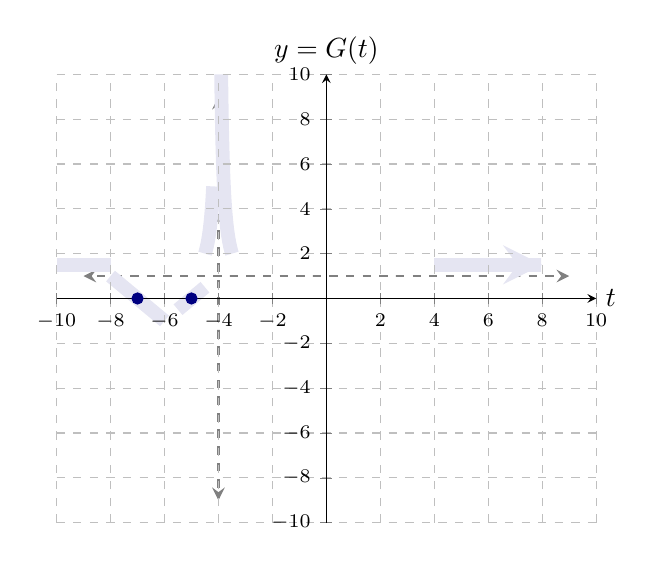
\begin{tikzpicture}
  \begin{axis}[
            domain=-10:10, ymax=10, xmax=10, ymin=-10, xmin=-10,
            axis lines =center, xlabel=$t$, ylabel={$y=G(t)$}, grid = major, grid style={dashed},
            ytick={-10,-8,-6,-4,-2,2,4,6,8,10},
            xtick={-10,-8,-6,-4,-2,2,4,6,8,10},
            yticklabels={$-10$,$-8$,$-6$,$-4$,$-2$,$2$,$4$,$6$,$8$,$10$}, 
            xticklabels={$-10$,$-8$,$-6$,$-4$,$-2$,$2$,$4$,$6$,$8$,$10$},
            ticklabel style={font=\scriptsize},
            every axis y label/.style={at=(current axis.above origin),anchor=south},
            every axis x label/.style={at=(current axis.right of origin),anchor=west},
            axis on top
          ]
          
          	\addplot [line width=1, gray, dashed,samples=200,domain=(-9:9),<->] {1};
          	\addplot [line width=1, gray, dashed,samples=200,domain=(-9:9),<->] ({-4},{x});



            \addplot [line width=5, penColor!10!background, smooth,samples=100,domain=(-8:-6)] {-(x+7)};
            \addplot [line width=5, penColor!10!background, smooth,samples=100,domain=(-5.5:-4.5)] {(x+5)};

            \addplot [line width=5, penColor!10!background, smooth,samples=100,domain=(-4.5:-4.2)] {-1/(x+4)};
            \addplot [line width=5, penColor!10!background, smooth,samples=100,domain=(-3.9:-3.5)] {1/(x+4)};



            \addplot [line width=5, penColor!10!background, smooth,samples=100,domain=(-10:-8)] {1.5)};
            \addplot [line width=5, penColor!10!background, smooth,samples=100,domain=(4:8),->] {1.5)};



          	\addplot[color=penColor,fill=penColor,only marks,mark=*] coordinates{(-7,0)};
          	\addplot[color=penColor,fill=penColor,only marks,mark=*] coordinates{(-5,0)};


           

  \end{axis}
\end{tikzpicture}
\end{image}









The graph is very suggestive that there is a local minimum somewhere around $-5.5$.  






\begin{image}
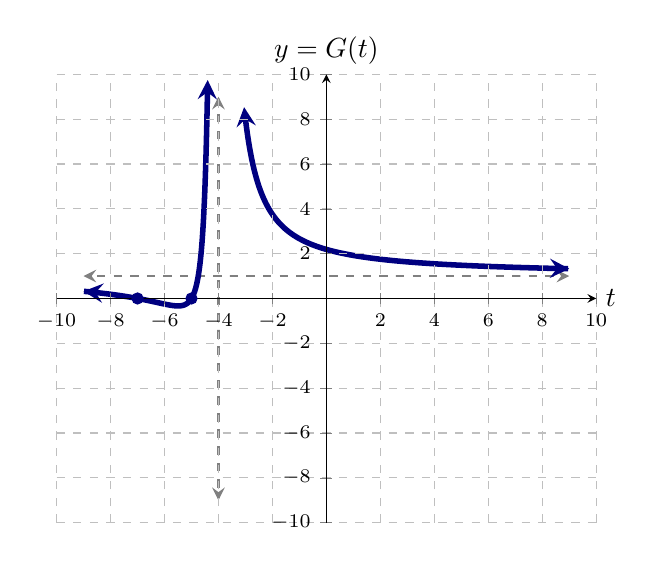
\begin{tikzpicture}
  \begin{axis}[
            domain=-10:10, ymax=10, xmax=10, ymin=-10, xmin=-10,
            axis lines =center, xlabel=$t$, ylabel={$y=G(t)$}, grid = major, grid style={dashed},
            ytick={-10,-8,-6,-4,-2,2,4,6,8,10},
            xtick={-10,-8,-6,-4,-2,2,4,6,8,10},
            yticklabels={$-10$,$-8$,$-6$,$-4$,$-2$,$2$,$4$,$6$,$8$,$10$}, 
            xticklabels={$-10$,$-8$,$-6$,$-4$,$-2$,$2$,$4$,$6$,$8$,$10$},
            ticklabel style={font=\scriptsize},
            every axis y label/.style={at=(current axis.above origin),anchor=south},
            every axis x label/.style={at=(current axis.right of origin),anchor=west},
            axis on top
          ]
          
            \addplot [line width=1, gray, dashed,samples=200,domain=(-9:9),<->] {1};
            \addplot [line width=1, gray, dashed,samples=200,domain=(-9:9),<->] ({-4},{x});


            \addplot [line width=2, penColor, smooth,samples=300,domain=(-9:-4.4),<->] {((x+7)*(x+5))/(x+4)^2};
            \addplot [line width=2, penColor, smooth,samples=300,domain=(-3.05:9),<->] {((x+7)*(x+5))/(x+4)^2};


            \addplot[color=penColor,fill=penColor,only marks,mark=*] coordinates{(-7,0)};
            \addplot[color=penColor,fill=penColor,only marks,mark=*] coordinates{(-5,0)};


           

  \end{axis}
\end{tikzpicture}
\end{image}

















\begin{center}
\desmos{st4dfylktg}{400}{300}
\end{center}





With some technology, we can approximate the critical number to be $-5.5$ and the local minimum to be $-0.333$, which agrees with our analysis.




The graph agrees with our analysis.


\end{explanation}






























\begin{center}
\textbf{\textcolor{green!50!black}{ooooo-=-=-=-ooOoo-=-=-=-ooooo}} \\

more examples can be found by following this link\\ \link[More Examples of Poynomial and Rational functions]{https://ximera.osu.edu/csccmathematics/precalculus/precalculus/polynomialFunctions/examples/exampleList}

\end{center}





\end{document}
